\section{Methodik und Ergebnisse}
\subsection{Methodisches Vorgehen und Ergebnisse der Programmierung}
\noindent Zur Auswertung der Kniebeugendaten aus der Phyphox-App werden zwei grafische Benutzeroberflächen (GUI) in \textit{MATLAB} programmiert. Dabei kommt die Version R2022a von \textit{MATLAB} zum Einsatz.

\subsubsection{Ablauf des Matlab-Programm Kalibrierungs\_GUI}
Die entsprechende GUI kann unter folgendem Link heruntergeladen werden:
  \href{https://raw.githubusercontent.com/pia-GUI/Kalibrierungs-GUI/refs/heads/main/Kalibrierung_GUI.m?token=GHSAT0AAAAAADBPPXZYMYTFDYPMM6UFDB42Z7L2ZPQ}{\texttt{Kalibrierung\_GUI.m}}
Im folgenden sieht man den Programmablaufplan der Kalibrierungs-GUI.
\usetikzlibrary{shapes.geometric, arrows.meta, positioning}

\tikzstyle{startstop} = [rectangle, rounded corners, minimum width=3cm, minimum height=1cm,text centered, draw=black, fill=gray!20]
\tikzstyle{process} = [rectangle, minimum width=3cm, minimum height=1cm, text centered, draw=black, fill=blue!20]
\tikzstyle{decision} = [diamond, minimum width=3.5cm, minimum height=1.5cm, text centered, draw=black, fill=orange!20, aspect=2]
\tikzstyle{arrow} = [thick,->,>=stealth]

\begin{tikzpicture}[node distance=1.4cm and 2.5cm]

\node (start) [startstop] {Start GUI};
\node (GUI) [process, below of =start] {Hauptfigur \& Komponenten (Button \& Achsen) erstellen}
\node (loadBtn) [process, below of=GUI] {Button \texttt{CSV-Dateien laden} drücken -> Callback startet};
\node (chooseFiles) [process, below of=loadBtn] {2 CSV-Dateien auswählen};
\node (cancelCheck) [decision, below of=chooseFiles] {Abbruch?};
\node (loadData) [process, right of=cancelCheck, xshift=5cm] {Daten einlesen mit \texttt{readtable}};
\node (syncAccel) [process, below of=loadData] {Synchronisation über Ruck (max. Beschleunigung)};
\node (synTime) [process, below of=syncAccel] {Gemeinsamen Zeitbereich bestimmen}
\node (calcAngle) [process, below of=synTime] {Berechne Neigungswinkel mit \texttt{atan2d} \& Glättung};
\node (interp) [process, below of=calcAngle] {Interpolation auf gemeinsamen Zeitvektor};
\node (kneeAngle) [process, below of=interp] {Kniewinkel = 180 - |Oberschenkel - Unterschenkel|};
\node (removeStart) [process, below of=kneeAngle] {Entferne Zeit < -3s};
\node (plot) [process, below of=removeStart] {Plotten des Winkels und 90°-Linie};
\node (end) [startstop, below of=plot] {Ende};

% Verbindungen
\draw [arrow] (start) -- (GUI);
\draw [arrow] (GUI) -- (loadBtn);
\draw [arrow] (loadBtn) -- (chooseFiles);
\draw [arrow] (chooseFiles) -- (cancelCheck);
\draw [arrow] (cancelCheck) -- node[above] {Nein} (loadData);
\draw [arrow] (loadData) -- (syncAccel);
\draw [arrow] (syncAccel) -- (synTime);
\draw [arrow] (synTime) -- (calcAngle);
\draw [arrow] (calcAngle) -- (interp);
\draw [arrow] (interp) -- (kneeAngle);
\draw [arrow] (kneeAngle) -- (removeStart);
\draw [arrow] (removeStart) -- (plot);
\draw [arrow] (plot) -- (end);
\draw [arrow] (plot) -- (end);
\draw [arrow] (cancelCheck.west) -- ++(0,-0.0) node[above] {Ja}  -- ++(-3.5,0) -- ++(0,5.55) -- (start.west);

\end{tikzpicture}
\noindent Zunächst werden die Hauptfigur und die Komponenten erstellt. Dabei werden Positionen, Größen und Bezeichnungen definiert.
\noindent Anschließend folgt die Funktion loadCSVCallback, die beim Drücken des Buttons „CSV-Dateien laden“ aufgerufen wird. Sie umfasst das Laden, Verarbeiten und Plotten der Messdaten. Mithilfe der vorgefertigten MATLAB-Funktion uigetfile kann der Anwender zwei CSV-Dateien vom Computer auswählen, eine für den Oberschenkel und eine für den Unterschenkel.
\begin{lstlisting}[style=Matlab-editor]
[file1, path1] = uigetfile('*.csv', 'CSV-Datei für Unterschenkel wählen');
[file2, path2] = uigetfile('*.csv', 'CSV-Datei für Oberschenkel wählen');
\end{lstlisting}
\\
\noindent Wird der Dateidialog abgebrochen oder werden fehlerhafte Dateien ausgewählt, wird der Vorgang beendet. Falls das Laden jedoch erfolgreich ist, werden die Daten mithilfe der vorgefertigten MATLAB-Funktion readtable als Tabellen in MATLAB eingelesen.

\begin{lstlisting}[style=Matlab-editor]
unterschenkel = readtable(fullfile(path1, file1));
oberschenkel = readtable(fullfile(path2, file2));
\end{lstlisting}
\\
\noindent Um die beiden Datensätze miteinander zu synchronisieren, wird zunächst die Differenz der Absolutbeschleunigungen berechnet. Anschließend wird jeweils der Index mit dem maximalen Beschleunigungsunterschied bestimmt. Diese Zeitpunkte werden genutzt, um die Zeitachsen so zu verschieben, dass beide Signale zeitgleich starten.
\noindent Aus dem überlappenden Bereich der Zeitachsen wird ein gemeinsamer Zeitvektor erstellt. Anschließend erfolgt die Berechnung des Kniegelenkwinkels. Dafür werden die Neigungswinkel der Sensoren auf Oberschenkel und Unterschenkel mithilfe der vorgefertigten MATLAB-Funktion atan2d berechnet, wobei jeweils die X- und Y-Komponenten der Beschleunigung verwendet werden. Die so gewonnenen Winkelverläufe werden geglättet, um Störungen zu reduzieren.
\begin{lstlisting}[style=Matlab-editor]
theta_unter = smoothdata(atan2d(unterschenkel.AccelerationY_m_s_2_, unterschenkel.AccelerationX_m_s_2_), 'movmean', 5);
theta_oben  = smoothdata(atan2d(oberschenkel.AccelerationY_m_s_2_, oberschenkel.AccelerationX_m_s_2_), 'movmean', 5);
\end{lstlisting}
\\
\noindent Es folgt eine Interpolation der geglätteten Winkelverläufe auf den gemeinsamen Zeitvektor, damit die Daten direkt miteinander vergleichbar sind. 
\begin{lstlisting}[style=Matlab-editor]
theta_unterschenkel_interp = interp1(unterschenkel.Time_Sync, theta_unter, common_time, 'linear', 'extrap');
theta_oberschenkel_interp  = interp1(oberschenkel.Time_Sync, theta_oben, common_time, 'linear', 'extrap');
\end{lstlisting}
\\
\noindent Aus der Differenz beider Winkel wird schließlich der Kniegelenkwinkel berechnet, indem diese Differenz von 180° subtrahiert wird. Der Wert 180° entspricht einer vollständigen Kniestreckung.
\begin{lstlisting}[style=Matlab-editor]
kniewinkel = 180 - abs(theta_oberschenkel_interp - theta_unterschenkel_interp);
\end{lstlisting}
\\
\noindent Nach der Berechnung des Kniegelenkwinkels werden die Anfangssegmente entfernt, da diese für die spätere Auswertung nicht benötigt werden. Anschließend erfolgt das Plotten des Kniegelenkwinkels zusammen mit einer Referenzlinie bei 90° als Vergleich.

\noindent Die folgende Abbildung 8 zeigt die Oberfläche der Kalibrierungs-GUI. Oben links befindet sich der Button zum laden der Daten. Nach Auswertung der Daten erscheint in dem darunterliegendem Diagramm der gemessene Winkel verlauf. 
\begin{figure}[ht]\centering
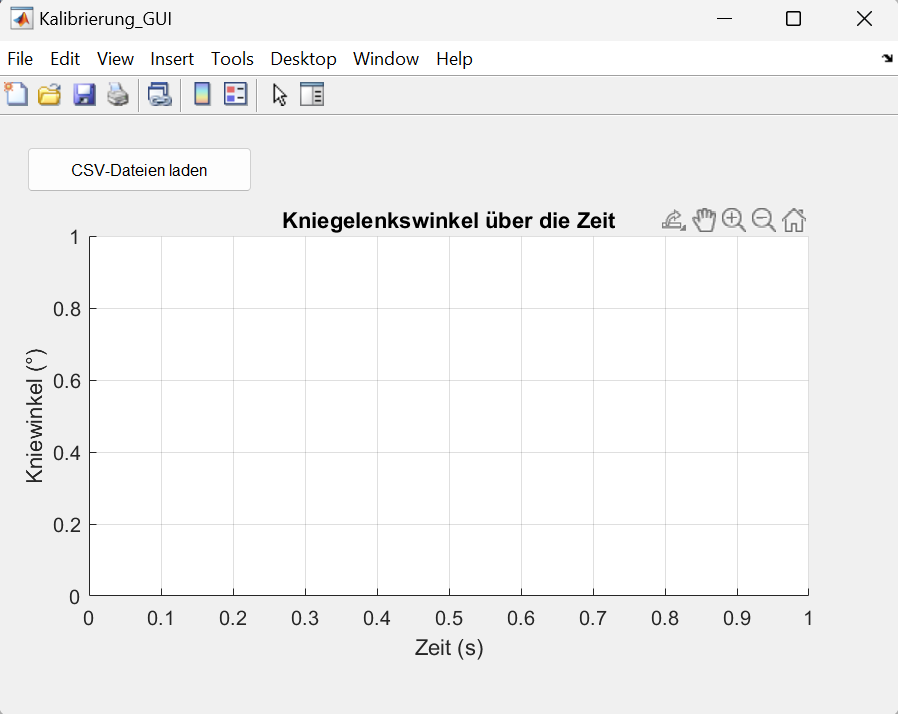
\includegraphics[width=0.75\linewidth]{images/Kalibrierung_GUI.png}
\caption{Oberfläche der Kalibierungs GUI}
\label{fig:Kalibrierungs GUI}
\end{figure}
\newpage
\subsubsection{Ablauf des Matlab-Programm KniewinkelAnalyse\_GUI}
\noindent Im Folgenden ist der Programmablaufplan der Kniewinkel-Analyse-GUI dargestellt. Die einzelnen Funktionen werden anschließend detailliert erklärt.

\noindent Die Kniewinkel-Analyse-GUI dient der Analyse des Kniegelenkwinkels anhand von CSV-Dateien. Die GUI besteht aus drei aufeinanderfolgenden Fenstern. Das erste GUI-Fenster ermöglicht die Auswahl der Kniebeugentiefe sowie die Eingabe der Probanden-ID.

\noindent Nach Betätigung des OK-Buttons wird die Callback-Funktion InfoGUI aufgerufen. In dieser Funktion werden die Informationstexte zu den verschiedenen Auswahlmöglichkeiten integriert sowie die Schwellenwerte gesetzt. Die Informationen zu den Schwellenwerten, der Probanden-ID und der ausgewählten Kniebeugen-Art werden anschließend an die nächste Funktion übergeben.

\noindent Für das dritte GUI-Fenster werden zunächst die Figur und die zugehörigen Komponenten erstellt.

\noindent Die verschiedenen Buttons sind mit Funktionen verknüpft. Zunächst wird der Button „CSV-Dateien laden“ betätigt, woraufhin die Funktion loadCSVCallback aufgerufen wird. Diese Funktion beinhaltet die gleichen Code-Komponenten wie die entsprechende Funktion in der Kalibrierung\_GUI.

\noindent Die Funktion SliderCallback setzt die Slider entsprechend des ausgewählten Schwellenwerts und speichert diesen, um ihn im weiteren Verlauf verwenden zu können.

\noindent Die Funktion updatePlot wird verwendet, um den Verlauf des Kniegelenkwinkels über die Zeit darzustellen. Zudem werden durch diese Funktion die gestrichelten Linien der Schwellenwerte eingefügt sowie die Minima bzw. die maximale Tiefe der Kniebeuge identifiziert. Hierfür wird die vorgefertigte MATLAB-Funktion findpeaks eingesetzt.

\begin{lstlisting}[style=Matlab-editor]
[~, locs] = findpeaks(-kniewinkel, 'MinPeakDistance', 130, 'MinPeakProminence', 25);
valid_times_minima = common_time(locs);
valid_minima = kniewinkel(locs);
\end{lstlisting}
\\
\noindent Die Anzahl der Kniebeugen innerhalb und außerhalb der Schwellenwerte wird zusätzlich berechnet und farblich im Plot markiert. Außerdem erfolgt eine Berechnung des durchschnittlichen Kniewinkels anhand der Minima, wozu die vorgefertigte MATLAB-Funktion mean verwendet wird.
\begin{lstlisting}[style=Matlab-editor]
average_minimum = mean(valid_minima);
\end{lstlisting}
\\
\noindent Zusätzlich gibt es ein Infofeld, in dem Informationen nach der Auswertung angezeigt werden. Dazu gehören die Probanden-ID, die Gesamtzahl der Kniebeugen, die Anzahl der Kniebeugen innerhalb der Schwellenwerte, die Anzahl der Kniebeugen oberhalb und unterhalb der Schwellenwerte sowie der durchschnittliche Kniegelenkswinkel.

\noindent Die letzte Funktion ist mit dem Speicher-Button verknüpft und heißt saveResultsCallback. Diese Funktion ermöglicht das Speichern der textlichen Rückmeldungen als Textdatei, wobei ein beliebiger Speicherort ausgewählt werden kann. Außerdem erfolgt eine Rückmeldung, ob das Speichern erfolgreich war oder nicht.
\begin{center}
\begin{tikzpicture}[node distance=1.4cm and 4cm, every node/.style={align=center}, >=stealth]

% Styles definieren
\tikzstyle{startstop} = [rectangle, rounded corners, minimum width=4.2cm, minimum height=1cm,text centered, draw=black, fill=gray!20]
\tikzstyle{KAG} = [rectangle, minimum width=5.0cm, minimum height=1.1cm, text centered, draw=black, fill=pink!20]
\tikzstyle{info} = [rectangle, minimum width=5.0cm, minimum height=1.1cm, text centered, draw=black, fill=yellow!10]
\tikzstyle{LMG} = [rectangle, minimum width=5.0cm, minimum height=1.1cm, text centered, draw=black, fill=purple!20]
\tikzstyle{load} = [rectangle, minimum width=5.0cm, minimum height=1.1cm, text centered, draw=black, fill=cyan!10]
\tikzstyle{save} = [rectangle, minimum width=5.0cm, minimum height=1.1cm, text centered, draw=black, fill=green!10]
\tikzstyle{plot} = [rectangle, minimum width=5.0cm, minimum height=1.1cm, text centered, draw=black, fill=blue!10]
\tikzstyle{schw} = [rectangle, minimum width=5.0cm, minimum height=1.1cm, text centered, draw=black, fill=orange!20]


% GUI-Teil
\node (start) [startstop] {Start Oberfläche mit Komponenten erstellen};
\node (auswahl) [KAG, below of=start] {Kniebeugen-Typ wählen};
\node (tiefe) [KAG, right=of auswahl, xshift=0.2cm] {Tiefe Kniebeuge};
\node (halbe) [KAG, below of=tiefe] {Halbe Kniebeuge};
\node (viertel) [KAG, below of=halbe] {Viertel Kniebeuge};
\node (spezial) [KAG, below of=viertel] {Spezielle Kniebeuge};

\node (id) [KAG, below of=auswahl] {Probanden-ID eingeben};
\node (OK) [KAG, below of=id] {OK Button}
\node (info) [startstop, below of=OK] {Info-Oberfläche};
\node (infotext) [info, below of=info] {Infotext anzeigen};
\node (schwelle) [info, below of=infotext] {Schwellwerte setzen};
\node (OK2) [info, below of=schwelle] {OK Button}
\node (start2) [startstop, below of=OK2] {Auswertung Oberfläche};
\node (3GUI) [LMG, below of=start2] {Komponenten erstellen und mit Funktionen verknüpfen};

% Hauptlinie
\node (csv) [load, below of=3GUI] {CSV-Dateien laden Button};
\node (schwell) [schw, below of=csv] {Schwellwerte übernehmen};
\node (plot) [plot, below of=schwell] {Kniewinkelverlauf + Schwellen + Minima plotten};
\node (auswertung) [plot, below of=plot] {Kniebeugen analysieren:\\ Anzahl und Bewertung};
\node (speichern) [save, below of=auswertung] {Auswertung als Text speichern};
\node (ende) [startstop, below of=speichern] {Ende};

% Rechte Abzweigung ab CSV-Dateien laden
\node (loadData) [load, right=of csv, xshift=0.01cm] {Daten einlesen mit \texttt{readtable}};
\node (syncAccel) [load, below of=loadData] {Zeit synchronisieren\\ über Beschleunigungsmaximum};
\node (calcAngle) [load, below of=syncAccel] {Neigungswinkel mit \texttt{atan2d}};
\node (interp) [load, below of=calcAngle] {Interpolation auf gemeinsamen Zeitvektor};
\node (kneeAngle) [load, below of=interp] {Kniewinkel berechnen};
\node (removeStart) [load, below of=kneeAngle] {Zeitraum $<$ 2s entfernen};

% Hauptflüsse
\draw [arrow] (start) -- (auswahl);
\draw [arrow] (auswahl) -- (tiefe);
\draw [arrow] (auswahl) -- (id);
\draw[arrow](id) -- (OK);
\draw [arrow] (tiefe) -- (halbe);
\draw [arrow] (halbe) -- (viertel);
\draw [arrow] (viertel) -- (spezial);
\draw [arrow] (OK) -- (info);
\draw [arrow] (info) -- (infotext)
\draw [arrow] (infotext) -- (schwelle);
\draw[arrow] (schwelle) -- (OK2)
\draw [arrow] (OK2) -- (start2);
\draw [arrow] (start2) -- (3GUI);
\draw[arrow] (3GUI) -- (csv)
\draw [arrow] (csv) -- (schwell)
\draw [arrow] (schwell) -- (plot);
\draw [arrow] (plot) -- (auswertung);
\draw [arrow] (auswertung) -- (speichern);
\draw [arrow] (speichern) -- (ende);

% Rechte Abzweigung von CSV
\draw [arrow] (csv) -- (loadData);
\draw [arrow] (loadData) -- (syncAccel);
\draw [arrow] (syncAccel) -- (calcAngle);
\draw [arrow] (calcAngle) -- (interp);
\draw [arrow] (interp) -- (kneeAngle);
\draw [arrow] (kneeAngle) -- (removeStart);

\end{tikzpicture}
\end{center}

\noindent Die Abbildung 9 zeigt die Oberfläche zur Auswahl des Kniebeugentyps. Über den Pfeil können die verschiedenen Optionen ausgewählt werden. Darunter kann im Textfeld die Probanden-ID eingegeben werden.
\begin{figure}[ht]\centering
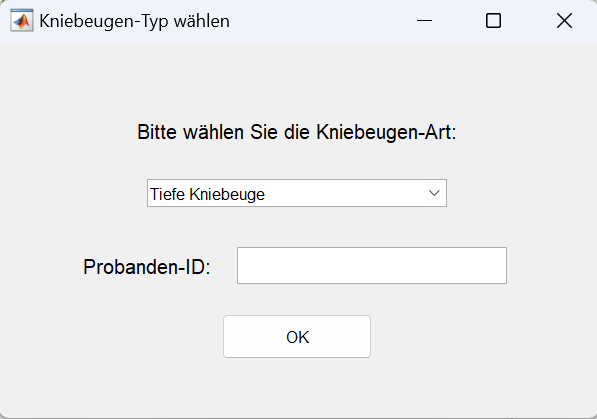
\includegraphics[width=0.75\linewidth]{images/Auswahl_GUI.png}
\caption{Oberfläche der Auswahl des Kniebeugentypes}
\label{fig:Kalibrierungs GUI}
\end{figure}
\noindent \noindent Die nächste Abbildung 10 zeigt die Oberfläche der Auswertungs-GUI. Oben links befindet sich der Button zum Laden der Daten. Rechts daneben werden die gesetzten Schwellenwerte angezeigt, welche bei Bedarf angepasst werden können.
\noindent Nach der Auswertung der Daten erscheint im darunterliegenden Diagramm der gemessene Winkelverlauf. Außerdem erfolgt oberhalb des Diagramms eine textliche Rückmeldung.
\noindent Über den oben rechts liegenden Button kann die textliche Auswertung, inklusive der Probanden-ID, als \texttt{.txt}-Datei abgespeichert werden.
\begin{figure}[ht]\centering
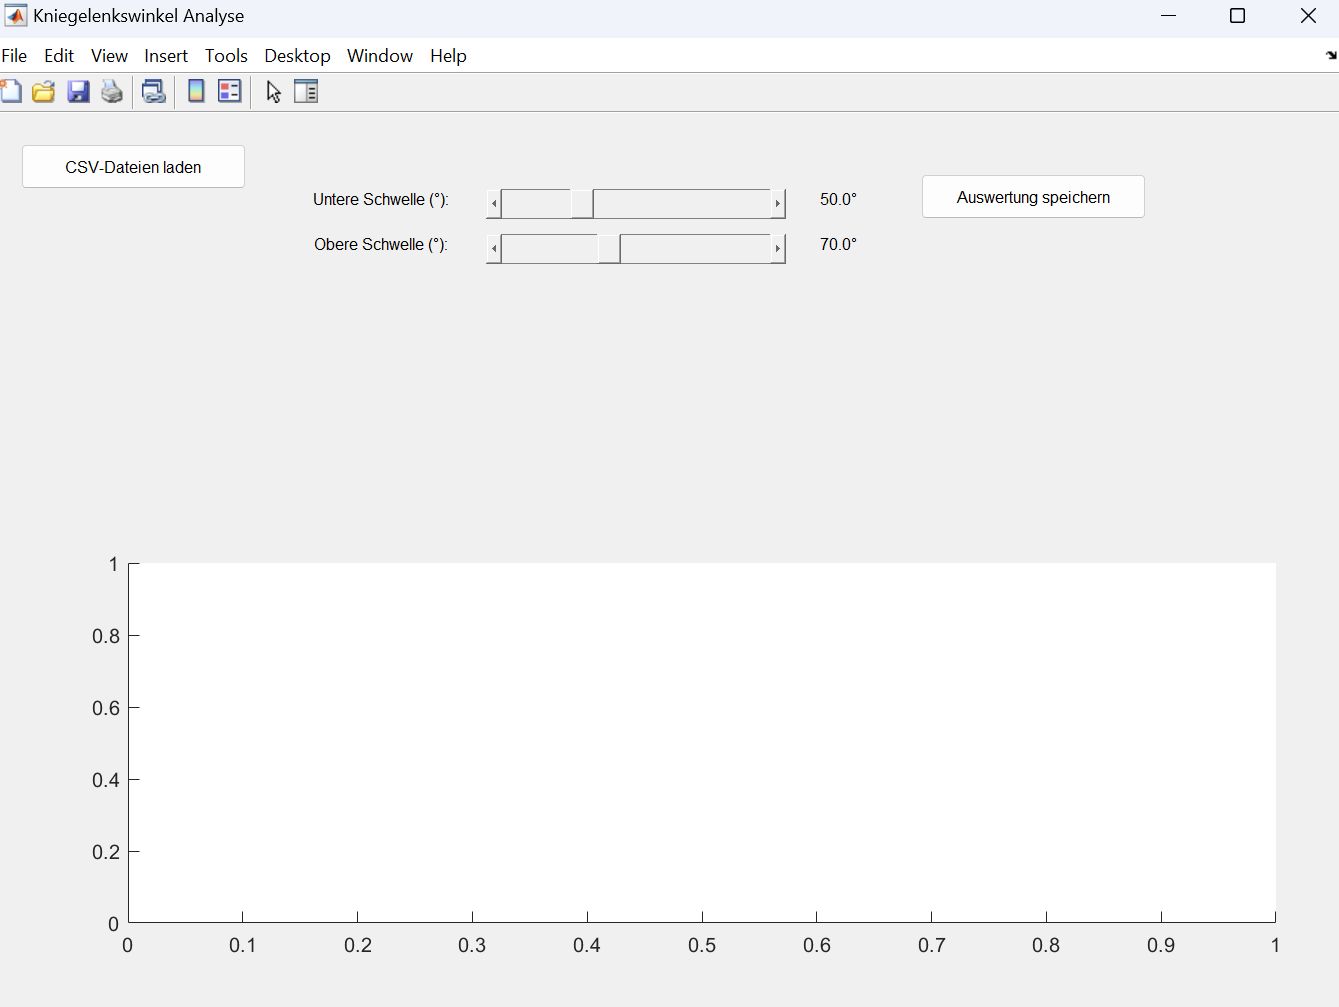
\includegraphics[width=0.75\linewidth]{images/Auswertungs_GUi.png}
\caption{Oberfläche der Auswertungs GUI}
\label{fig:Kalibrierungs GUI}
\end{figure}

\subsection{Versuchsdurchführung}
\noindent Im folgenden wird die Datenaufnahme in Phyphox und die anschließende Daten Auswertung erklärt. Anhand dieser Anleitung kann der Anwender Schritt für Schritt den Ablauf nachvollziehen und selber durchführen.

\noindent Das Ziel der entwickelten Anwendung ist die eigenständige Auswertung und Bewertung der Ausführung einer Kniebeuge hinsichtlich des Kniegelenkwinkels. Abhängig von verschiedenen Ausführungsvarianten wird bei der Kniebeuge ein unterschiedlicher Kniegelenkswinkel erwartet. 

\subsubsection{Einleitung und Zielsetzung}
Ziel des Versuchs ist die präzise Messung und Analyse des Kniegelenkwinkels bei der Durchführung von Kniebeugen mit unterschiedlichen Bewegungstiefen. Dabei soll überprüft werden, inwiefern die Versuchsperson die vorgegebenen Zielbereiche des Kniewinkels (tiefe, halbe und viertel Kniebeuge) einhalten kann. Die Auswertung erfolgt über eine eigens entwickelte MATLAB-GUI, die auf Basis der aufgezeichneten Sensordaten den Verlauf des Kniewinkels graphisch und textlich darstellt.

\subsubsection{Material und Geräte}
\begin{itemize}
    \item Beliebige Umgebung möglich
    \item 2x Smartphones mit installierter Phyphox-App
    \item 1x Smartphone mit Videokamera
    \item 1x Stativ zur Kamerapositionierung
    \item Befestigungsgurte zur Fixierung der Smartphones an Unter- und Oberschenkel
    \item Sporttape zur Befestigung
    \item 1x Winkelmesser
    \item 1x Stuhl, höhenverstellbar
    \item PC mit installierter Analyse-Software (KnieAngleGUI)
\end{itemize}

%% Für die GUI auch Links hinzufügen um die Runterzuladen 

\subsubsection{Technische Vorbereitung}
Für die Durchführung des Versuchs werden drei Smartphones benötigt, von denen zwei mit der Phyphox-App ausgestattet sind. Diese Geräte dienen der Messung der Beschleunigung an Oberschenkel und Unterschenkel. Das dritte Smartphone wird zur Videoaufzeichnung eingesetzt. Zusätzlich wird ein PC mit der installierten Auswertungssoftware benötigt. Vor Beginn des Versuchs werden alle Geräte eingeschaltet, die Phyphox-App vorbereitet und das Videoaufnahmegerät startklar gemacht. Der PC wird hochgefahren, sodass im Anschluss die aufgezeichneten Daten verarbeitet werden können.

\subsubsection{Vorbereitung der Versuchsperson}
Vor Beginn der Messung wird das schriftliche Einverständnis der Versuchsperson eingeholt. Zusätzlich werden mögliche gesundheitliche Einschränkungen oder bekannte Pathologien erfragt, um potenzielle Risiken auszuschließen. Die Versuchsperson sollte enganliegende oder kurze Kleidung tragen, insbesondere an den Beinen, um eine möglichst körpernahe Befestigung der Smartphones zu gewährleisten und Störfaktoren zu minimieren. Im Anschluss wird der Ablauf des Versuchs kurz erläutert. (Weitere Details siehe Anhang: Probandenaufklärung zur Studie „Messung des Kniegelenkwinkels bei Kniebeugen mit verschiedenen Anforderungen“.)

\subsubsection{Versuchsaufbau}
Die Länge des Beins bis zum Knie wird gemessen, um den Stuhl auf die passende Höhe einzustellen. Anschließend werden die beiden Mess-Smartphones mit Befestigungsgurten am Bein fixiert. Ein Smartphone wird seitlich am Oberschenkel, das andere seitlich am Unterschenkel angebracht. Die genaue Platzierung platzierung der Smartphone ist von Bedeutung um eine korrekte Analyse zur erhalten. Die genauen Befestigungspunkte werden anhand der Abbildung ?? dargestellt. 
\\
\\
?????? Bild von der Befestigung
\\
\\
Vor Beginn der Datenaufnahme sollte überprüft werden, ob die Smartphones fest sitzen und keine Bewegungseinschränkung verursachen.
\noindent Das dritte Smartphone wird auf einem Stativ in der Sagittalebene auf Höhe des Knies positioniert, um die Bewegung aufzuzeichnen.

\subsubsection{Kalibrierungsmessung}
\noindent Um die Daten der Phyphox-App korrekt auszuwerten, sollten vor der Aufnahme einige Vorbereitungen getroffen werden. Zur Kalibrierung wird zunächst ein Video gestartet und beide Phyphox-Apps geöffnet. Unter dem Sensor-Menüpunkt „Beschleunigung mit g“ wird die Messung möglichst gleichzeitig gestartet. Das Starten der Aufnahme erfolgt über den *Play*-Button in der oberen orangenen Leiste. Dies kann entweder von der Testperson selbst oder von einer helfenden Person durchgeführt werden. Falls das annähernd gleichzeitige Starten nicht gelingt, kann der Datensatz einfach über das "Mülltonnen-Symbol" gelöscht und die Aufnahme erneut gestartet werden. Sobald die Aufnahme läuft, kann die Durchführung der Übung beginnen.
\noindent Um beide Datensätze bei der Auswertung synchronisieren  zu können, sollte zu Beginn einen markanter Punkt in den Daten sichtbar sein. Am einfachsten ist es, das Bein einmalig ruckartig nach oben zu Bewegung. Dieser Ruck kann im Programm in beiden Datensätzen erkannt werden und ermöglicht so die exakte Synchronisierung. Danach setzt sich die Person ruhig auf den zuvor eingestellten Stuhl. 
\noindent Der Kniewinkel im Sitzen wird mit einem Winkelmesser überprüft und bei Bedarf manuell korrigiert, bis ein Winkel von 90° erreicht ist. Die Person bleibt etwa 10 Sekunden lang ruhig in dieser Position. Anschließend wird die Messung pausiert und das Video gestoppt.
\noindent Die aufgezeichneten Sensordaten werden als CSV-Dateien im Format „Comma, decimal point“ exportiert und sinnvoll benannt (z.B. Probemessung\_---\_1\_Oberschenkel). Die Daten werden auf dem Laptop gespeichert und in der KnieAngleGUI geladen. Dort erfolgt eine automatische Synchronisation und Berechnung des Kniewinkels. Liegt dieser nicht im Bereich von 90° ±5, wird die Kalibrierung durch erneutes Anpassen der Smartphone-Positionen wiederholt.

\subsubsection{Versuchsdurchführung}
\noindent Die Versuchsperson führt nacheinander drei Kniebeugenserien mit unterschiedlicher Zieltiefe durch:
\begin{itemize}
    \item Tiefe Kniebeugen (Kniewinkel zwischen 40° und 60°)
    \item Halbe Kniebeugen (Kniewinkel zwischen 80° und 100°)
    \item Viertel Kniebeugen (Kniewinkel zwischen 110° und 140°) \cite{Hartmann2014}
\end{itemize}
\noindent In den folgenden Abbildungen wird die Ausführungstiefe der verschiedenen Ausführungsvarianten Bildlich dargestellt. 
\\
\\
?????? Bilder für die Ausführungstiefe
\\
\\
\noindent Für jede der drei Serien (tiefe, halbe und viertel Kniebeuge) wird ein einheitlicher Ablauf durchgeführt. Zunächst wird das Video auf dem dritten Smartphone gestartet, und die aktuelle Uhrzeit wird notiert, um eine eindeutige Zuordnung der Daten zu ermöglichen. Anschließend wird auf beiden Phyphox-Geräten die Messung gleichzeitig gestartet. Zur Synchronisation der Sensoraufzeichnungen mit dem Video führt die Versuchsperson erneut einen kurzen Ruck mit dem Bein aus.
\noindent Daraufhin werden zehn Kniebeugen in der jeweils vorgegebenen Zieltiefe durchgeführt. Nach Abschluss der Bewegungsausführung sollte die Testperson ruhig stehen bleiben und die Messung wird  über die Phyphox-App gestoppt und das Video beendet. Die dabei aufgezeichneten Sensordaten werden anschließend als CSV-Dateien im Format „Comma, decimal point“ exportiert. Dazu wird in der oberen orangenen Leiste das Drei-Punkte-Menü ausgewählt. Nun kann eine Aktion ausgewählt werden in diesem Fall der Datenexport. Es ist darauf zu achten, dass die Dateien eindeutig und nachvollziehbar benannt werden – zum Beispiel Tiefe\_---\_Oberschenkel oder Halbe\_---\_Unterschenkel. Diese Dateien dienen als Grundlage für die spätere Auswertung in der Analyse-Software. 

\subsubsection{Datenauswertung}
\noindent Nach Abschluss aller Serien wird die KnieAngleGUI auf dem PC geöffnet. Dort wählt man die jeweilige Kniebeugenart aus und lädt die entsprechenden CSV-Dateien. Die Anwendung synchronisiert die Daten und berechnet den zeitlichen Verlauf des Kniewinkels.
\noindent Die Ergebnisse werden grafisch dargestellt. Kniebeugen, deren tiefster Punkt innerhalb des definierten Zielbereichs liegt, werden grün markiert. Abweichungen außerhalb des Zielbereichs erscheinen rot. Zusätzlich wird eine schriftliche Auswertung generiert, die folgende Informationen enthält: Gesamtanzahl der Kniebeugen, Anzahl der Kniebeugen innerhalb des Schwellwertbereichs, Anzahl der zu tiefen Kniebeugen, Anzahl der zu hohen Kniebeugen. 

\noindent (Weitere Details siehe Anhang: Versuchsprotokoll Kniebeugen) 

\subsubsection{Ergebnisse der Untersuchung}

